Accurately modelling a wide variety of functions allows to impute missing values and create continuous data for further processing. This is necessary for empirical real world data, where gaps between discrete measurements need to be filled. 

One example from the field of astronomy are brightness values from cepheid variable stars. Cepheid stars change their luminosity periodically, as visible in \autoref{fig:cepheid_image}. Crucially, as discovered by the astronomer Henrietta Leavitt, the frequency of those periods directly correlates to their absolute luminosity. Knowing the absolute luminosity of a star is very useful, as it allows astronomers to calculate the distance to that star. Early in the 20th century there was an ongoing debate, whether the andromeda galaxy, formerly known as andromeda nebula, is part of our own galaxy or rather a galaxy of its own. By discovering cepheid variable stars in the andromeda galaxy and using Leavitts Law, the distance to the andromeda galaxy could be calculated and the andromeda galaxy was recognized as such. \cite{gaßnerAstroBook}

\begin{figure}[h]
	\centering
	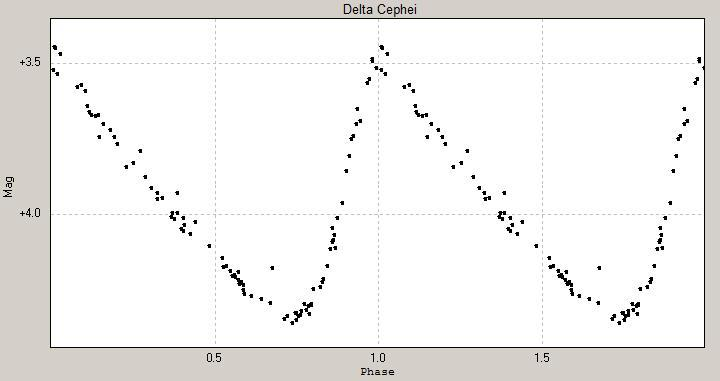
\includegraphics[width = 0.5\textwidth]{figures/Cephei}
	\caption{Phase lightcurve of variable star Delta Cephei \tiny\url{ https://de.wikipedia.org/wiki/Datei:Delta_Cephei_lightcurve.jpg}}
	\label{fig:cepheid_image}
\end{figure}

Estimating the underlying function given the provided data in \autoref{fig:cepheid_image} would allow to remove the present noise and apply further processing like calculating extrema of that function and computing the frequency based on that. 

We sample synthetic time series data from a multivariate normal distribution and train a transformer model to estimate unseen values given a certain number of context points. We follow the general approach from \citet{seifner2025zeroshotimputationfoundationinference}, while using transformers instead of LSTMs and estimating the actual function, instead of derivatives.